% File project.tex
%% Style files for ACL 2021
\documentclass[11pt,a4paper]{article}
\usepackage[hyperref]{acl2021}
\usepackage{times}
\usepackage{booktabs}
\usepackage{todonotes}
\usepackage{latexsym}
\renewcommand{\UrlFont}{\ttfamily\small}
\usepackage{multirow}

% This is not strictly necessary, and may be commented out,
% but it will improve the layout of the manuscript,
% and will typically save some space.
\usepackage{microtype}

\aclfinalcopy 

\newcommand\BibTeX{B\textsc{ib}\TeX}

\title{11-777 Spring 2021 Class Project}

\author{
  Christian Deverall\thanks{\hspace{4pt}Everyone Contributed Equally -- Alphabetical order} \hspace{2em} Jingyuan Li $^*$ \hspace{2em} Artidoro Pagnoni $^*$ \\
  \texttt{\{cdeveral, jingyua4, apagnoni\}@andrew.cmu.edu}
  }

\date{}

\begin{document}
\maketitle

\section{Introduction and Problem Definition}
Understanding and following task-oriented instructions are natural and straightforward skills for human races, while this remains to be a great challenge for robotic systems, due to the difficulties in both visual and linguistic understanding. In this project, we are interested in allowing the robots to understand the instructions and take actions based on the instructions, like what the human race would do. As a result, the ALFRED dataset \cite{ALFRED20} was chosen for this project.

The high-level task for the ALFRED dataset is to predict the correct sequence of household actions given textual instructions and visual feedback. The ALFRED dataset is unique in that the actions are long, compositional, and non-reversible. An example of this is that the agent must pick up a knife in order to slice a potato. Moreover, once a potato is sliced, it cannot be put back together. Actions consist of navigation within a room or interaction with an object. For interaction, a pixelwise mask must be predicted whereby the object with the highest intersection-over-union score with the interaction mask is acted upon. The textual instructions come in the form of both high-level task descriptions and step by step commands. The visual feedback is ego-centric and the next image is provided after each action is performed. Compared to previous datasets, there is a diverse range of tasks. Specifically there are 7 high-level task types parameterized by a combination of 84 object classes and 120 household scenes.

In this project, the focus will be on the navigation and interaction of the agent in the simulator. The Input space would be a set of instructions (represented in natural language) and an image (represented in ResNet-18 \cite{He_2016_CVPR} features) reflecting the current environment perceived by the agent. The output space is the prediction of the next action that helps the agent achieve the ultimate goal. The predicted actions can be described in three dimensions, including 1) a classification outcome indicating the type of action, 2) the magnitude of action when the action is for navigation, and 3) an object mask indicating the location of an object acted on when the objects are involved in the action. The input image is updated for the next prediction after an action is performed. To evaluate the success of the prediction sequence, the number of desired state changes in the target object completed by the agent is measured.

\begin{table}[]
    \centering
    \resizebox{\linewidth}{!}{
\begin{tabular}{lrrrr}
\toprule
     split &  mean &  std &  min &  max \\
\midrule
    low-level train &  49.78 & 24.78 &    5 &   234 \\
    low-level val seen &  46.98 & 20.22 &    13 &   137 \\
    low-level val unseen & 50.12 & 25.61 &    12 &   165\\
    high-level train &  6.51 & 2.49 &  2 &   19 \\
    high-level val seen &  6.47 & 2.62 &    3 &   16 \\
    high-level val unseen &  6.16 & 2.33 &    3 &   14 \\
\bottomrule
\end{tabular}
}
    \caption{Statistics on the number of low-level and high-level actions for the splits of the data.}
    \label{tab:number_actions}
\end{table}

\section{Data Analysis}
We present an analysis of the data. Our objective is to get a sense of the types of examples that are present in the dataset. The sizes of the seen validation set, unseen validation set and training set are 251, 255 and 6574 respectively.

\subsection{Action Space Analysis}

In the ALFRED dataset, tasks are described by low-level and high-level actions. In this section, we examine the patterns behind these actions and the objects which are acted upon. In order to gauge the size of tasks and the granularity of actions, we provide statistics about the number of low-level and high-level actions per task in \autoref{tab:number_actions}.

Low-level actions are often repeated in order to fully complete a high-level goal. For example, numerous fixed-distance movement actions are required to travel from one end of the kitchen to the other. This repetition pattern is relevant to action prediction because for highly repeated actions, it is likely that the next action is the exact same as the current one. In \autoref{fig:duplicate_dist}, it can be seen that by far the most duplicated action is the "MoveAhead" operation encompassing approximately 44\% of all actions.

\begin{figure}
    \centering
    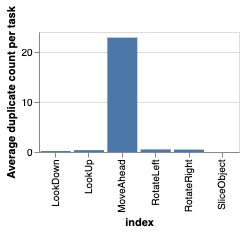
\includegraphics[width=\linewidth]{Reports/1-Task-Definition-and-Data/duplicate_distrib.png}
    \caption{Average number of duplicate actions per task}
    \label{fig:duplicate_dist}
\end{figure}

To further understand the sequential order of actions, we display the distribution of next actions given current actions in \autoref{fig:heatmap_act}. Only data from the training split is shown here. Current actions are shown on the left axis while next actions are shown on the bottom axis. The top three most common sequences of actions are "MoveAhead" then "MoveAhead", "RotateLeft" then "MoveAhead" and "RotateRight" then "MoveAhead".
\begin{figure*}
    \centering
    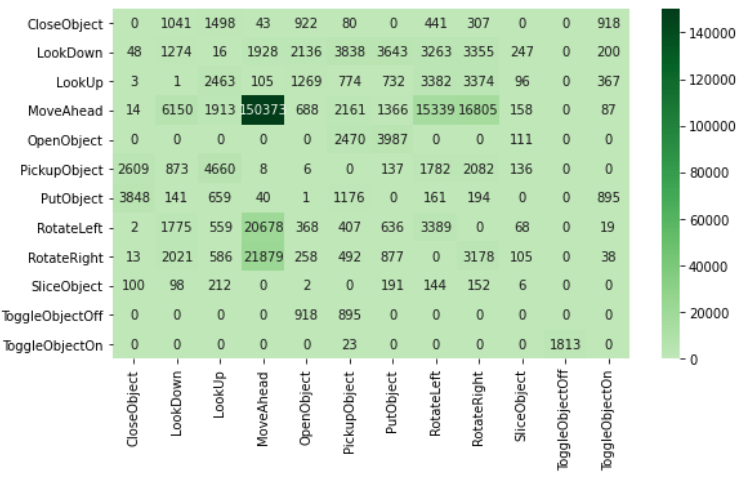
\includegraphics[width=\linewidth]{Reports/1-Task-Definition-and-Data/heatmap_actions.png}
    \caption{Heatmap to show the frequency of low-level action bigrams in the training set.}
    \label{fig:heatmap_act}
\end{figure*}

Objects are utilized in two manners. They are acted upon or they are decorative in that they exist in the room but are not used. To get a sense of the distribution of the acted upon objects, we plot the top 20 most used objects in \autoref{fig:used_obj}. The microwave and fridge are used far more frequently than other objects. This is most likely because they are highly common household items that essential for "OpenObject" and "CloseObject" actions. The distribution of all objects regardless of whether they are used or not is shown in \autoref{fig:all_obj}.

\begin{figure}
    \centering
    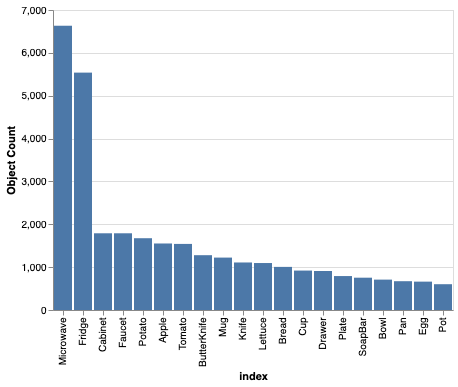
\includegraphics[width=\linewidth]{Reports/1-Task-Definition-and-Data/used_objects.png}
    \caption{The frequency distribution of objects used within actions.}
    \label{fig:used_obj}
\end{figure}

\begin{figure}
    \centering
    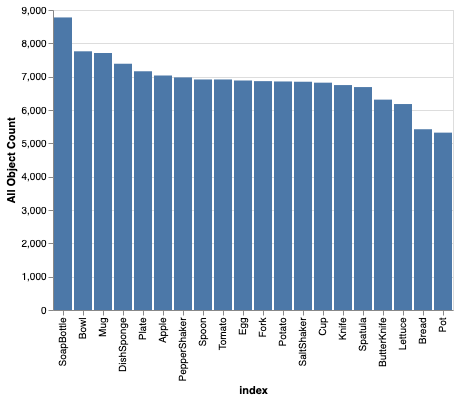
\includegraphics[width=\linewidth]{Reports/1-Task-Definition-and-Data/all_obj.png}
    \caption{The frequency distribution of all objects.}
    \label{fig:all_obj}
\end{figure}

Certain objects are more frequently used for certain actions. Intuitively, a potato is more likely to be sliced than a microwave. Thus, to understand which objects are more frequently used for each action, we plot an action-object heatmap in \autoref{fig:act_obj}.

\begin{figure*}
    \centering
    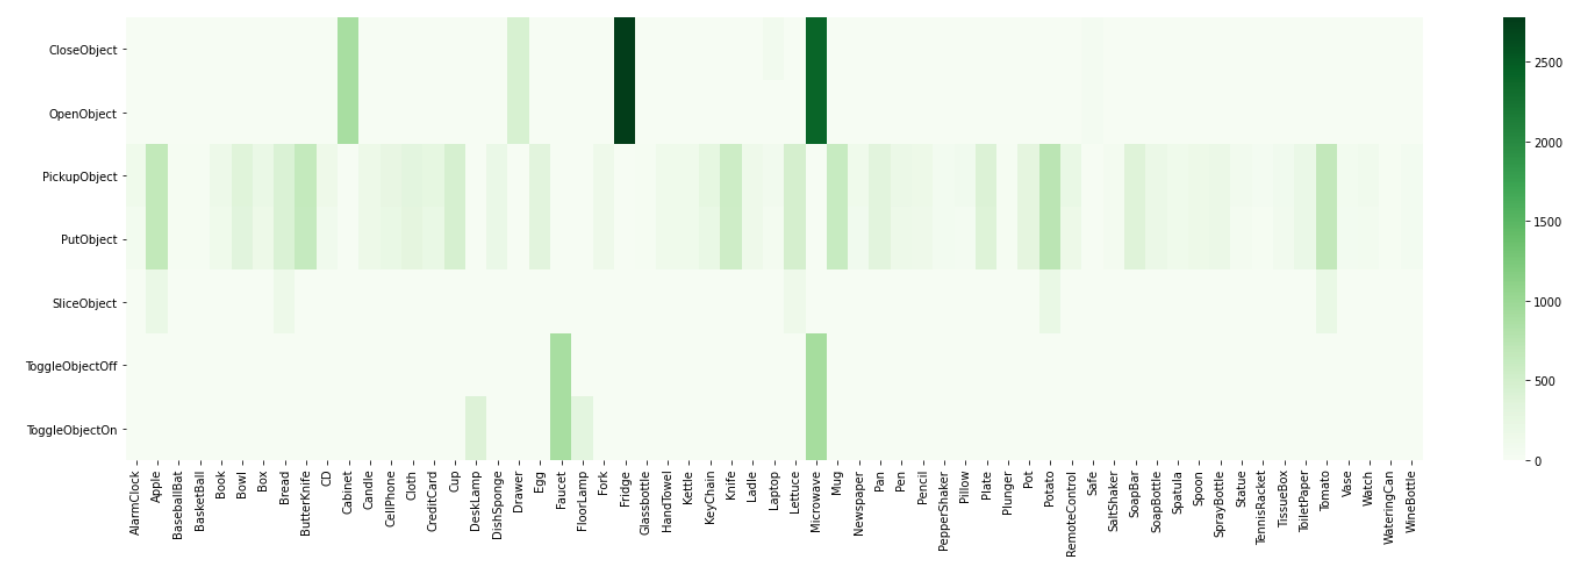
\includegraphics[width=\linewidth]{Reports/1-Task-Definition-and-Data/act_obj.png}
    \caption{A heatmap to show which object is utilized more frequently for each action.}
    \label{fig:act_obj}
\end{figure*}

\subsection{Instructions Analysis}
There are two types of instructions: the task description and the detailed instructions. The task description is generally a single sentence outlining the goal of the task while the detailed instructions break the task down in sub-goals and provide a sentence instruction for each sub-goal. We measure statistics on the number of sub-goal for each task in \autoref{tab:sub_goals}. We observe that there are up to 19 different sub-goals in each trajectory and that on average there are 6.7. The tasks are not simple as they require a minimum of three sub-goals.

\begin{table}[]
    \centering
\begin{tabular}{lrrrr}
\toprule
     split &  mean &  std &  min &  max \\
\midrule
     train &  6.72 & 2.49 &    3 &   19 \\
  val seen &  6.79 & 2.73 &    4 &   16 \\
val unseen &  6.26 & 2.33 &    4 &   14 \\
\bottomrule
\end{tabular}
    \caption{Statistics on the number of sentence instructions (sub-goals) for the splits of the data.}
    \label{tab:sub_goals}
\end{table}


There are different sets of each instruction for each trajectory. We examine the statistics of the number of separate sets of instructions for each trajectory in \autoref{tab:instruction_sets}. We observe that there are generally three sets for each trajectory, but they can go up to six.

\begin{table}[]
    \centering
    \begin{tabular}{lrrrr}
    \toprule
         split &  mean &  std &  min &  max \\
    \midrule
         train &  3.20 & 0.68 &    3 &    6 \\
      val seen &  3.27 & 0.80 &    3 &    6 \\
    val unseen &  3.22 & 0.72 &    3 &    6 \\
    \bottomrule
    \end{tabular}
    \caption{Statistics on the number sets of instructions for each trajectory by split.}
    \label{tab:instruction_sets}
\end{table}

When inspecting the instructions we notice that verbs indicate actions, while nouns indicate objects. We measure statistics on the number of verbs and nouns in both types of instructions. In both cases, we use the lemma of the noun and verb. We report the results in \autoref{tab:verbs_nouns_stats}. The number of verbs used can go as high as 68 verbs for one set of detailed instructions. On average the number of verbs is around 13 in the detailed instructions and slightly over one in the task instructions. 

Besides the actual values, we observe that the ratio of nouns to verbs is higher in the task instructions. This indicates that in the task instructions there are more complements used to specify the actions described by the verbs. By manual analysis, the task instructions have specifications on the location where an action should be completed. This is information that comes in addition to the object that needs to be acted on and makes the sentence structure more complex. 

It is surprising that some task instructions do not contain any nouns. We inspected some of the sentences without nouns and they seem to be truncated sentences for example: ``The ro''. This indicates that there is some noise in the data.


\begin{table*}[]
    \centering
\begin{tabular}{llrrrr|rrrr}
\toprule
        & & \multicolumn{4}{c|}{Nouns} & \multicolumn{4}{c}{Verbs}\\
    Instruction Type & split &  mean &  std &  min &  max &  mean &  std &  min &  max \\
\midrule
\multirow{3}{*}{Task Instructions}
&      train &  3.08 & 1.10 &    0 &   10 &  1.26 & 0.53 &    0 &    8 \\
&   val seen &  3.09 & 1.16 &    0 &   11 &  1.28 & 0.58 &    0 &    5 \\
& val unseen &  3.09 & 1.16 &    0 &   11 &  1.28 & 0.58 &    0 &    5 \\
\midrule
\multirow{3}{*}{Detailed Instructions}
&      train & 19.89 &  9.15 &    2 &   98 & 13.13 & 6.81 &    1 &   68 \\
&   val seen & 19.89 & 10.16 &    5 &   82  & 12.98 & 7.31 &    2 &   53 \\
& val unseen & 19.89 & 10.16 &    5 &   82  & 12.98 & 7.31 &    2 &   53 \\
\bottomrule
\end{tabular}
    \caption{Statistics on the number of verbs and nouns in the instructions for each split.}
    \label{tab:verbs_nouns_stats}
\end{table*}

In order to get a sense of the type of objects and verbs that appear in the instructions, we plot their distributions. In both cases they are long tailed distributions with most of the elements occurring very rarely. The distribution over verbs is steeper than that over nouns. This partly relates to the fact that there are fewer action types than objects in the ALFRED world. We do also notice that there are a lot of synonyms in both cases. For example, in the verbs, both ``turn'' and ``veer'' are present. These two verbs are very close in meaning.

\begin{figure}
    \centering
    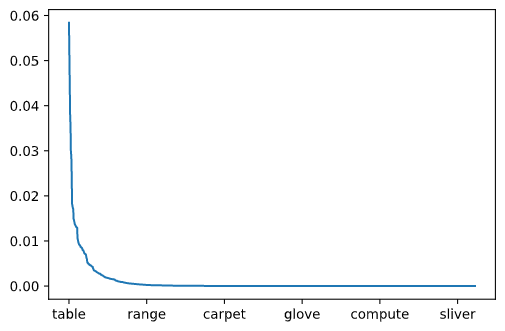
\includegraphics[width=\linewidth]{Reports/1-Task-Definition-and-Data/train_noun_dist.png}
    \caption{Frequency of occurrences of nouns in the detailed instructions in the training set.}
    \label{fig:nouns_train}
\end{figure}

\begin{figure}
    \centering
    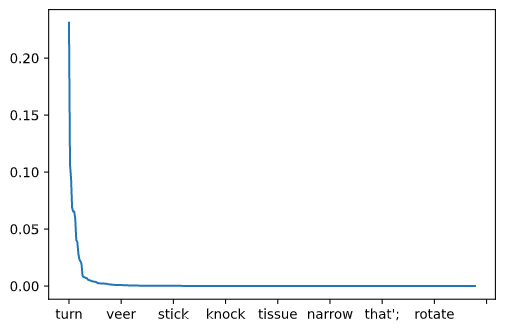
\includegraphics[width=\linewidth]{Reports/1-Task-Definition-and-Data/train_verb_dist.png}
    \caption{Frequency of occurrences of verbs in the detailed instructions in the training set.}
    \label{fig:nouns_train}
\end{figure}

We compare the occurrence of objects in the instructions between the training and validation set to estimate how often there will be unseen objects in the test set. We observe that there are only 22 unobserved objects in the validation set that did not appear in the training set.  When looking at verbs, we only observe 6 verbs that appeared in the validation sets but not in the training set. This is relatively small and not surprising since the set of actions remains the same across the two splits. In both cases, the proportion of unseen objects and verbs is lower than $0.1\%$ so it should not be of major concern.


We also look at the actions that generally follow each other. To this end we build a confusion matrix of pairs of verbs in \autoref{fig:matrix_verbs}. We study how verbs follow each other in the instructions. In general, we observe that the most frequent pairs of verbs involve navigation. The interactive actions are less frequent, and they appear after other navigation actions (like ``face'' or ``walk''). 

\begin{figure*}
    \centering
    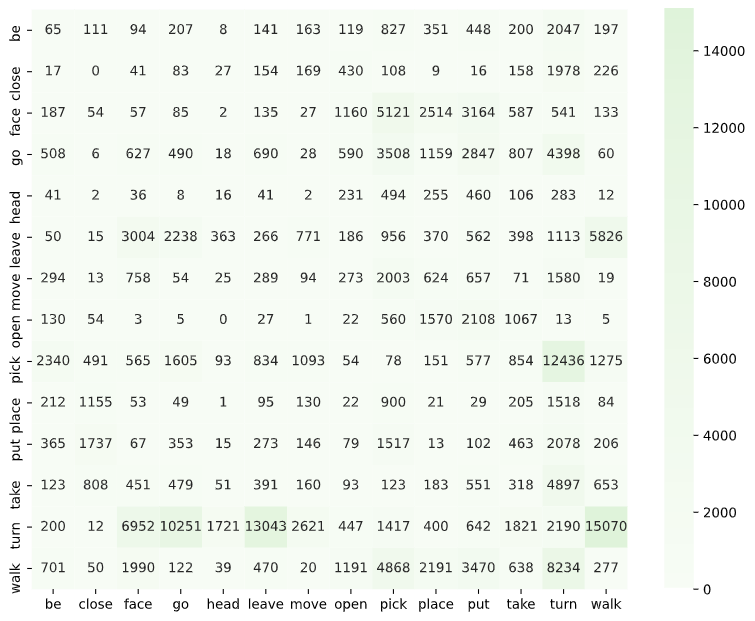
\includegraphics[width=\linewidth]{Reports/1-Task-Definition-and-Data/matrix_verbs.png}
    \caption{Occurrence of verbs following each other. Only displaying the most frequent verbs.}
    \label{fig:matrix_verbs}
\end{figure*}


\section{Conclusion}
In this report, we analyze the ALFRED \cite{ALFRED20} dataset. We explore both the actions and the instructions in the training and validation data splits.


\clearpage
% Please use 
\bibliographystyle{acl_natbib}
\bibliography{references}

%\appendix



\end{document}
